\chapter{仿真实验与分析}
\label{chap:experiment}

在上一章节中介绍本文的三种预测算法,在本章节中我们将针对这三种预测模型分别进行实验仿真来验证我们的算法的准确率。此外,由于在实验环境当中很难获取到真实的LTE定位数据,我们将采用使用第二章节中提到的人群模拟算法进行数据生成,本文中提到的预测算法是针对特大城市的聚集事件进行研究,所以我们将最基本的人群模拟模型即可满足需求,所以我们选择基于社会关系的人群模拟模型生成实验数据。在生成实验数据之后我们将分别使用拟合、基于相邻区域特征的GBDT算法和基于自动编码器隐藏特征的GBDT算法进行预测,预测目标为未来1到10个时刻的人群密度。在得到这些预测结果后,我们根据第三章提到的误差计算公式来评价各个算法的正确率。

\section{实验数据生成}

仿真软件选择Pedsim2.3。Pedsim软件不仅提供模拟行人移动的功能,而且将仿真模块和模拟算法进行了分离,能够方便的扩展和定制。示例如\ref{fig:ped2d}和\ref{fig:ped3d}所示:

\begin{figure}[!htp]
    \centering
    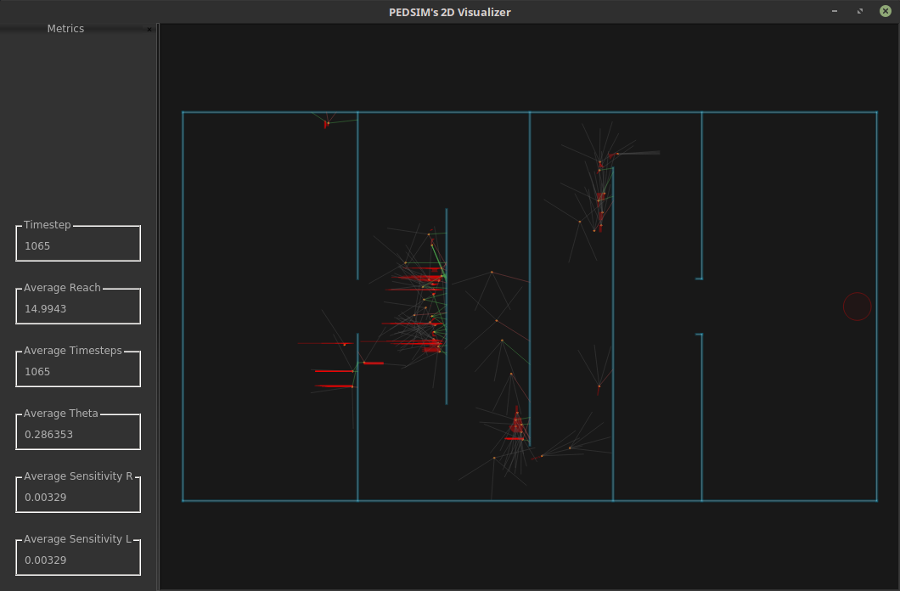
\includegraphics[width=0.6\textwidth]{chap4/ped2d}
    \bicaption[fig:ped2d]{Pedsim 2D仿真}{Pedsim 2D仿真}{Fig.}{Pedsim 2D Simulation}
\end{figure} 

\begin{figure}[!htp]
    \centering
    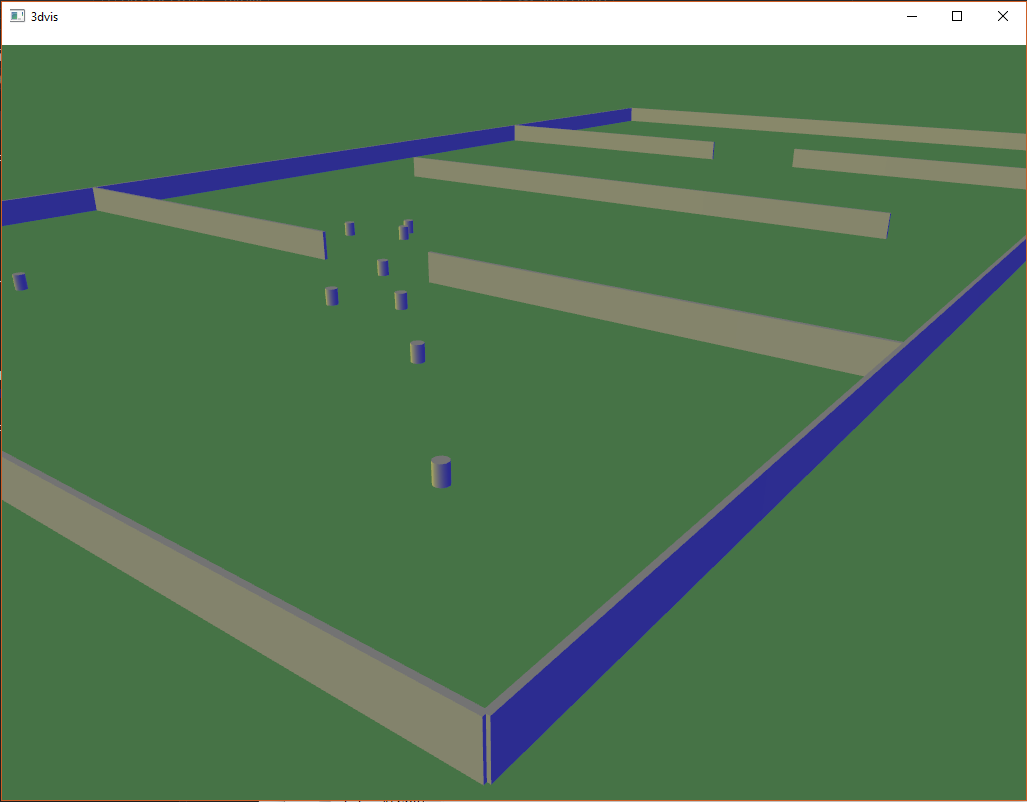
\includegraphics[width=0.6\textwidth]{chap4/ped3d}
    \bicaption[fig:ped3d]{Pedsim 3D仿真}{Pedsim 3D仿真}{Fig.}{Pedsim 3D Simulation}
\end{figure} 

模拟核心负责系统的物理模型,如行人代理与环境或彼此之间的交互等情况。这些问题的典型模拟技术有:
\begin{enumerate}
    \item 在微观模拟中,每个模拟行人的粒子都是独立的。
    \item 在宏观或基于场的模拟中,粒子聚集成场。相应的数学模型是偏微分方程,其需要对其计算以实现离散化。
    \item 有可能结合微观和基于场的方法,称为平滑粒子流体动力学(英文:smooth particle hydrodynamics,缩写:SPH)。在平滑粒子流体动力学中,保持每个颗粒的独立性。在每个时间步长内,颗粒聚集为场强度例如密度,然后从这些密度计算速度,然后根据这些宏观速度移动每个单独的颗粒。
    \item 作为第四种方法,在某种程度上,存在来自操作研究的排队模拟。这里粒子在队列的网络中移动,其中每个队列具有服务速率。一旦粒子被服务,它移动到下一个队列。
\end{enumerate}

对于Pedsim来说需要维护单个的粒子,因为这些粒子需要能够在整个模拟中做出独立的决策,例如路线选择。这立即排除基于场的方法。我们还需要一个现实的代表行人之间的交互,排除队列模型和平滑粒子流体动力学模型。

对于微观模拟,基本上有两种技术,分别是基于耦合微分方程的方法和元胞自动机(英文:cellular automata,缩写:CA)模型。在Pedsim仿真情况当中最重要的是每个行人可以在任意方向移动,而没有由建模技术造成的虚假位置,这本质上排除了元胞自动机技术。行人运动的一般耦合微分方程模型是社会力模型。

行人之间相互作用,包括避免碰撞,例如短距离相互作用和对路线交叉的行人的吸引力,这种远程的行为代表了行人的“意志“。这种对敌人的吸引力只是一个例子,应该被一些更复杂的和有意义的功能所替换。还实现了避免诸如树这种阻挡物的影响,这种行人移动模型也考虑到了建筑物的影响。此外建筑物内部的模拟是可能的,这允许使用相同的框架,例如人群疏散模拟。

任何移动性模拟系统不仅仅包括移动性模拟本身,对虚拟世界中的代理的物理约束,而且还包括计算代理的更高级别策略的模块。特别需要注意的一点是要完全分开地去考虑物理和心理世界。

\begin{enumerate}
    \item \textbf{物理层} \\ 负责系统的物理方面,例如代理的移动,代理与环境的交互或代理之间的交互。
    \item \textbf{精神层} \\ 部分的实现人类智力,这提高了代理行为的合理性。实际上,如果心理层策略非常复杂,在物理模拟中不需要社交力模型,即认为所有的力都可以设置为零。前瞻性心理策略告诉每个代理在他面前寻找其他代理,左边和右边的计数。然后它将走向更少的其他代理的方向。行人本身避免与墙壁和其他行人的碰撞,而不是由底层物理模型的约束。心理层模块的另一个例子是路由生成器。代理人随意走动是不够的,对于现实应用,有必要为每个行人产生合理的路线,能够计算路由,如路由生成器所做的,只有当知道代理的目的地时路由生成器才有意义。在交通研究中的一种技术是为每个代理人和每个活动的具体位置产生每天的活动链,存在非常复杂的心理层模块,例如,有一个视图分析器模块,它向系统描述当个体代理在景观中移动时“看到”什么。分析代理视场,并且向系统发送事件以描述代理看到什么。
\end{enumerate}

在本文的实验中我们搭建模拟上海市陈毅广场到人民广场地铁站一段的路况,并且设置陈毅广场、南京东路和人民广场三个热点,另外受硬件条件的限制我们不妨假设在地图中总共有400个行人,模拟图如\ref{fig:sim}所示。

\begin{figure}[!htp]
    \centering
    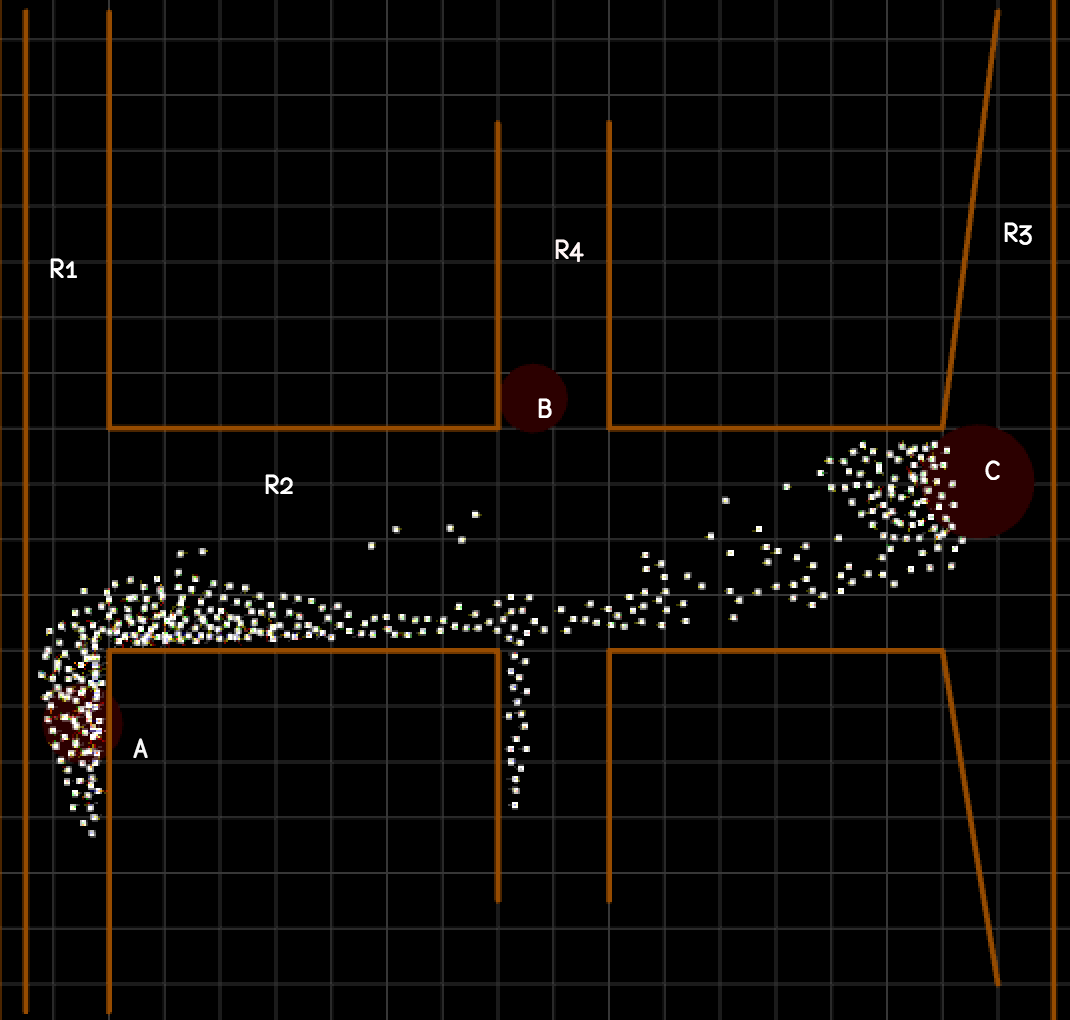
\includegraphics[width=0.8\textwidth]{chap4/sim}
    \bicaption[fig:sim]{数据生成}{数据生成}{Fig.}{Generate Data}
\end{figure} 
如图所示,其中A点视为人民广场地铁站、B点视为南京东路地铁站、C点为外滩陈毅广场,$R_1$为西藏南路、$R_2$为南京东路步行街、$R_3$为外滩沿线、$R_4$为河南中路。我们在初始阶段分别在A、B、C三个点分别设置120个行人,在河南中路末端设置40个行人,并且设置A、B两点的行人目的地为C点,C点中60人目的地为A点另外60人的目的地为B点,河南中路末端的40人的目的地也为C点。这样我们就模拟了这样一种场景:在外滩的活动之后一部分人群期望乘坐地铁回家,一部分人前往活动地点参加活动。我们的模拟过程从人群开始行动开始到所有行人均到达过C点结束。我们将这段时间行人的位置和时间记录下来,作为我们的仿真数据。

\section{仿真实验}

\subsection{实验环境}

\begin{enumerate}
    \item \textbf{硬件环境} \\
    处理器:2.4 GHz Intel Core i5 \\
    内存:8 GB 1600 MHz DDR3 \\
    硬盘:250GB 
    \item \textbf{软件环境} \\
    操作系统:macOS Sierra 10.12.1 \\
    开发工具:Vim8.0,Xcode 8.1,Matlab 2015b \\
    数据处理工具:Matlab \\
    Python解释器:2.7.6
    \item \textbf{其他第三方工具} 
    \begin{enumerate}
        \item \textbf{Matlab DeepLearnToolbox} \\
        DeepLearnToolbox\cite{IMM2012-06284}使用于深度学习的开发工具,提供了神经网络、自动编码器等函数库。
        \item \textbf{NumPy} \\ NumPy是Python的科学计算的基本包。其中包括:
        \begin{enumerate}
            \item 一个强大的N维数组对象
            \item 强大的函数库
            \item 用于集成C / C ++和Fortran代码的工具
            \item 有用的线性代数,傅立叶变换和随机数能力  
        \end{enumerate}
        除了其明显的科学用途,NumPy也可以用作通用数据的高效多维容器。 可以定义任意数据类型。 这允许NumPy无缝,快速地与各种各样的数据库集成。NumPy根据BSD许可证授权。
        \item \textbf{SciPy} \\ SciPy是一个基于Python的数学,科学和工程开源软件生态系统。它通过向用户提供用于操作和可视化数据的高级命令和类,为交互式Python会话增加了显着的功能。使用SciPy,交互式Python会话成为一个数据处理和系统原型开发环境,比如MATLAB,IDL,Octave,R-Lab和SciLab。
        
        基于SciPy对Python的额外的好处是,这也是一个强大的编程语言可用于开发复杂的程序和专门的应用程序。使用SciPy的科学应用程序受益于世界各地的开发人员在软件领域众多领域开发附加模块。从并行编程到Web和数据库子程序和类的一切都已经提供给Python开发人员。除了SciPy中的数学库之外,所有这些功能都可用。
        \item \textbf{Scikit-learn} \\ scikit-learn是Python的一个开源机器学习模块,它建立在NumPy,SciPy和matplotlib模块之上。值得一提的是,scikit-learn最先是由David Cournapeau在2007年发起的一个Google Summer of Code项目,从那时起这个项目就已经拥有很多的贡献者了,而且该项目目前为止也是由一个志愿者团队在维护着。有着以下的特点:
        \begin{enumerate}
            \item 简单高效的工具,用于数据挖掘和数据分析
            \item 可访问每个人,并可重复使用在各种情况下
            \item 基于NumPy,SciPy和matplotlib
            \item 开源,商业可用,使用BSD开源许可证
        \end{enumerate}
    \end{enumerate}
\end{enumerate}

\subsection{实验流程}

\begin{enumerate}
    \item \textbf{数据预处理} \\
    生成的数据中只包含行人的ID、定位信息、时间戳这三个基本数据,我们需要将数据处理成实验中能够识别的格式。按照第三章中提到的数据处理算法,我们将每个用户的定位信息做圆计算定位圆和小区方格相交区域的面积作为该用户在指定时间内出现在对应小区的概率,将每个小区所有行人出现的概率进行累加即可得到这个小区内的人群密度。并按照预测个数将数据分为训练数据和预测数据。
    \item \textbf{相邻区域特征提取} \\
    按照第三章中提到的算法,将待预测小区的人群密度和周围8个相邻的小区人群密度这9个特征作为相邻区域的特征。
    \item \textbf{自动编码器特征提取} \
    根据第二章中提到的神经网络和自动编码器理论,我们要将上一步中提取的到的9个特征同时作为输入和输出传入到神经网络当中,将神经网络当中学习到的特征作为数据源在下一步中进行预测。神经网络的特征我们进行如表\ref{tab:param}选取。   
    \begin{table}[!hpb]
        \centering
        \bicaption[tab:param]{神经网络训练参数}{神经网络训练参数}{Table}{}
        \begin{tabular}{@{}cc@{}} \toprule
            名称 & 参数 \\ \midrule
            隐藏层数 & 1 \\
            隐藏特征个数 & 15 \\
            训练次数 & 500 \\
            激活函数 & Sigm \\ \bottomrule
        \end{tabular}
    \end{table}
    \item \textbf{GBDT训练和测试} \\
    在选取好特征之后,使用GBDT回归模型将训练数据进行训练得到预测模型。将测试数据使用得到的预测模型进行计算,将预测得到的结果和正确的结果进行比较,使用第三章提到的结果比较算法我们将得到算法的预测正确率。
\end{enumerate}

\section{实验结果和分析}

使用多项式拟合正确率如表\ref{tab:poly-result}所示。

\begin{table}[!hpb]
    \centering
    \bicaption[tab:poly-result]{多项式拟合预测结果}{多项式拟合预测结果}{Table}{Polynomial Regression predict result}
    \begin{tabular}{@{}cc@{}} \toprule
        时间间隔 & 正确率 \\ \midrule
        1 &	4.49\% \\
        2 &	5.03\% \\
        3 &	5.82\% \\
        4 &	6.95\% \\
        5 &	7.69\% \\
        6 &	9.21\% \\
        7 &	10.69\% \\
        8 &	12.23\% \\
        9 &	12.07\% \\ 
        10 & 12.18\% \\
        \bottomrule
    \end{tabular}
\end{table}

使用相邻区域特征的GBDT算法正确率如表\ref{tab:gbdt}所示。

\begin{table}[!hpb]
    \centering
    \bicaption[tab:gbdt]{相邻区域特征预测结果}{相邻区域特征预测结果}{Table}{Neighbor Features predict result}
    \begin{tabular}{@{}cc@{}} \toprule
        时间间隔 & 正确率 \\ \midrule
        1 &	4.49\% \\
        2 &	5.03\% \\
        3 &	5.82\% \\
        4 &	6.95\% \\
        5 &	7.69\% \\
        6 &	9.21\% \\
        7 &	10.69\% \\
        8 &	12.23\% \\
        9 &	12.07\% \\ 
        10 & 12.18\% \\
        \bottomrule
    \end{tabular}
\end{table}

使用自动编码器提取特征的GBDT算法正确率如表\ref{tab:ac}所示。

\begin{table}[!hpb]
    \centering
    \bicaption[tab:ac]{自动编码器特征预测结果}{自动编码器特征预测结果}{Table}{Autoencoder predict result}
    \begin{tabular}{@{}cc@{}} \toprule
        时间间隔 & 正确率 \\ \midrule
        1 &	3.35\% \\
        2 &	9.71\% \\
        3 & 13.41\% \\
        4 &	13.50\% \\
        5 &	15.42\% \\
        6 &	16.33\% \\
        7 &	18.31\% \\
        8 & 18.46\% \\
        9 &	19.12\% \\
        10 & 19.26\% \\
        \bottomrule
    \end{tabular}
\end{table}

\section{本章小结}

在本章节中我们分别对本文提出的几种算法进行仿真实验,并对实验结果进行了对比,也对算法受时间的影响进行了分析。通过实验我们可以得到以下结论;
\begin{enumerate}
    \item 使用机器学习的算法能够对未来的人群密度进行较为准确的预测。
    \item 随着预测时间的增加,预测准确率逐步下降但准确率会平稳在一个固定水平。
    \item 使用自动编码器的算法性能还有待提升。
\end{enumerate}

三种算法的预测效果对比如图\ref{fig:compare}所示。

\begin{figure}[!htp]
    \centering
    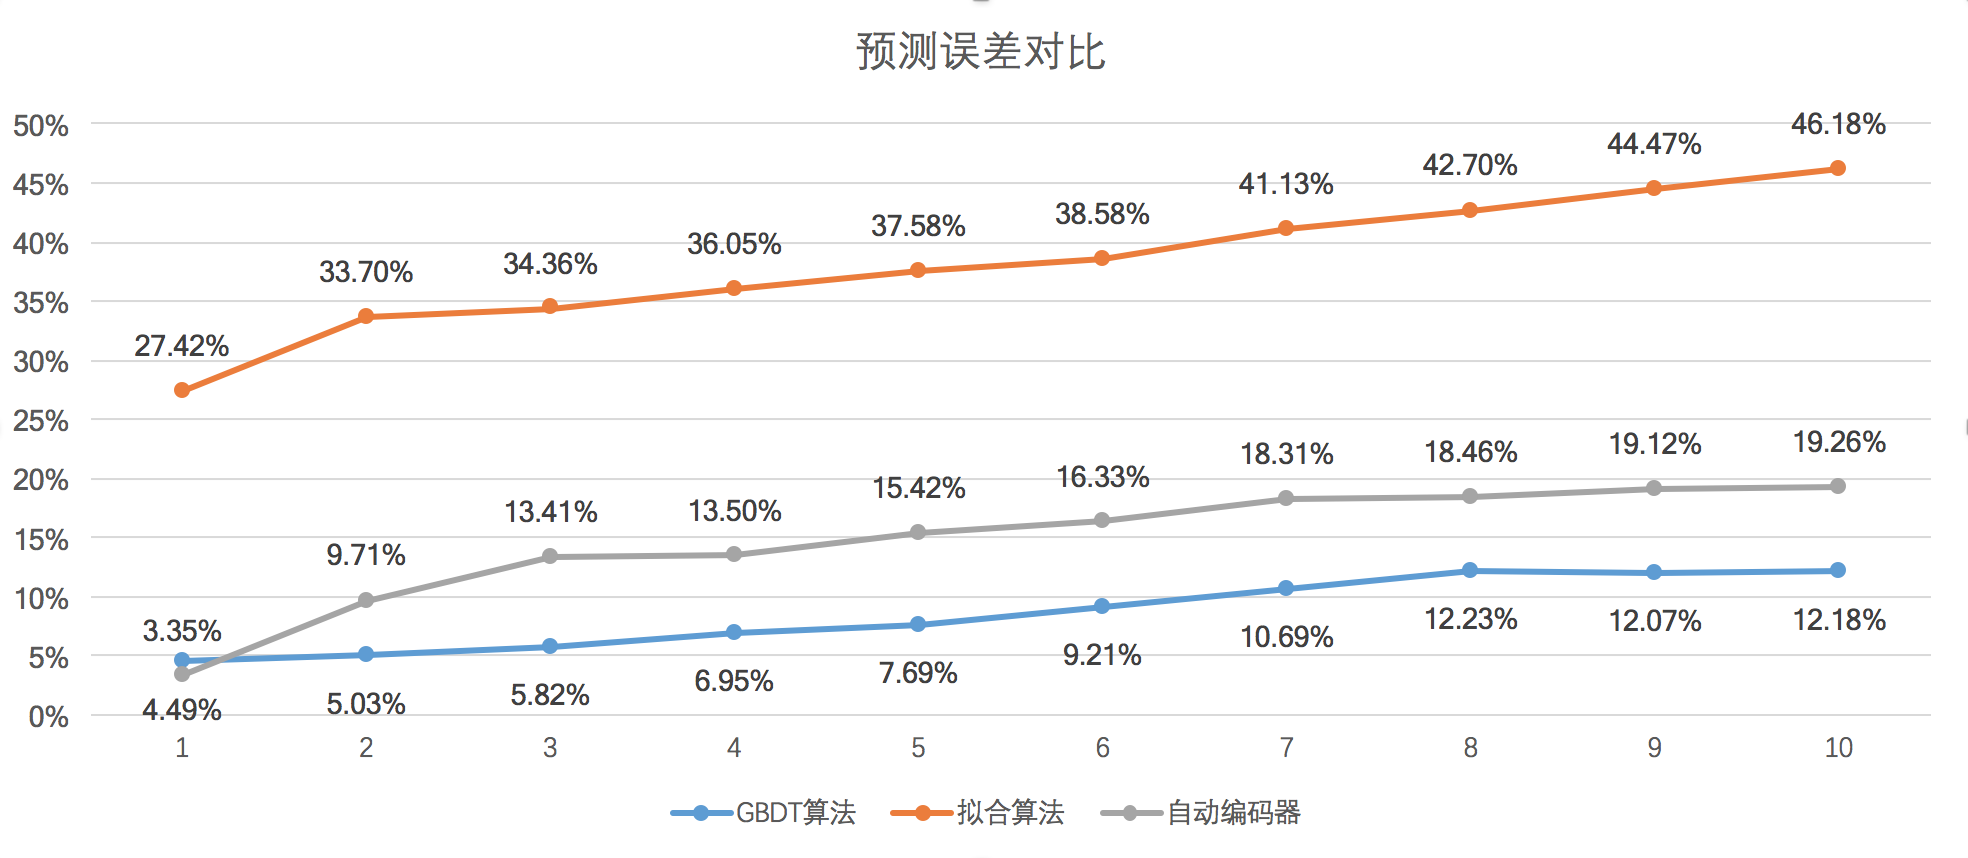
\includegraphics[width=0.8\textwidth]{chap4/compare}
    \bicaption[fig:compare]{实验结果对比}{实验结果对比}{Fig.}{Experiment result}
\end{figure} 